\begin{task}
Wyznacz współczynniki zespolonego szeregu fouriera dla okresowego sygnału $f(t)$ przedstawionego na rysunku 

\begin{figure}[H]
\centering
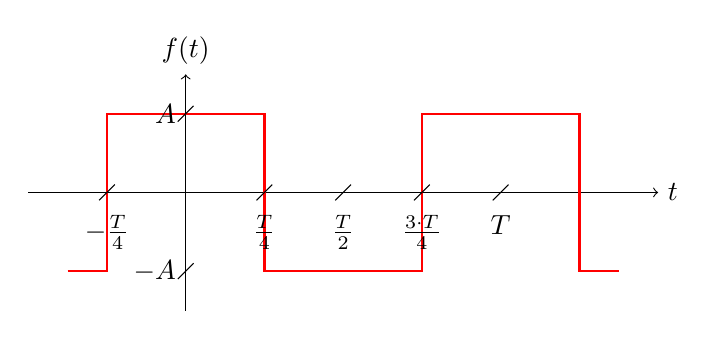
\begin{tikzpicture}
  %\draw (0,0) circle (1in);
  \draw[->] (-2.0,+0.0) -- (+6.0,+0.0) node[right] {$t$};
  \draw[->] (+0.0,-1.5) -- (+0.0,+1.5) node[above] {$f(t)$};
  \draw[-,red, thick] (-1.5,-1.0) -- (-1.0,-1.0) -- (-1.0,+1.0) -- (+1.0,+1.0) -- (+1.0,-1.0)--(+3.0,-1.0) -- (+3.0,+1.0) -- (+5.0,+1.0) -- (+5.0,-1.0) -- (+5.5,-1.0);
  %\draw[-] (-1.0-0.1,-0.1)--(-1.0+0.1,0.1) node[midway, below, outer sep=10pt,align=center] {$-\frac{T}{2}$};
  \draw[-] (-1.0-0.1,-0.1)--(-1.0+0.1,0.1) node[midway, below, outer sep=5pt,align=center] {$-\frac{T}{4}$};
  \draw[-] (+1.0-0.1,-0.1)--(+1.0+0.1,0.1) node[midway, below, outer sep=5pt] {$\frac{T}{4}$};
  \draw[-] (+2.0-0.1,-0.1)--(+2.0+0.1,0.1) node[midway, below, outer sep=5pt] {$\frac{T}{2}$};
  \draw[-] (+3.0-0.1,-0.1)--(+3.0+0.1,0.1) node[midway, below, outer sep=5pt] {$\frac{3\cdot T}{4}$};
  \draw[-] (+4.0-0.1,-0.1)--(+4.0+0.1,0.1) node[midway, below, outer sep=5pt] {$T$};
  \draw[-] (-0.1,+1.0-0.1)--(+0.1,+1.0+0.1) node[midway, left] {$A$};
  \draw[-] (-0.1,-1.0-0.1)--(+0.1,-1.0+0.1) node[midway, left] {$-A$};
\end{tikzpicture}
\end{figure}

W pierwszej kolejności należy opisać sygnał za pomocą wzoru.

\begin{equation}
   f(x)=\begin{cases}A & t \in \left (  0+k \cdot T; \frac{T}{2}+k \cdot T \right ) \\0 & t \in \left ( \frac{T}{2}+k \cdot T; T +k \cdot T\right )\end{cases} \wedge k \in C %\mathbb{C}
\end{equation}

Współczynnik $F_0$ wyznaczamy ze wzoru

\begin{equation}
F_0=\frac{1}{T}\int_{T}f(t) \cdot dt
\end{equation}

Podstawiamy do wzoru wzór naszej funkcji w pierwszym okresie $k=0$

\begin{equation}
\begin{aligned}
F_0 &=\frac{1}{T}\int_{T}f(t) \cdot dt =\\
&=\frac{1}{T} \left( \int_{0}^{\frac{T}{2}} A \cdot dt + \int_{\frac{T}{2}}^{T} 0 \cdot dt \right ) = \\
&=\frac{1}{T} \left( A \cdot \int_{0}^{\frac{T}{2}} dt + 0 \right ) = \\
&=\frac{1}{T} \left( A \cdot \left. t\right |_{0}^{\frac{T}{2}} \right ) = \\
&=\frac{A}{T} \cdot \left. t\right |_{0}^{\frac{T}{2}} = \\
&=\frac{A}{T} \cdot \left( \frac{T}{2} - 0 \right ) = \\
&=\frac{A}{T} \cdot \left( \frac{T}{2} \right ) = \\
&=\frac{A}{\cancel{T}} \cdot \left( \frac{\cancel{T}}{2} \right ) = \\
&=\frac{A}{2} 
\end{aligned}
\end{equation}

Wartość współczynnika $F_0$ wynosi $\frac{A}{2}$


Współczynnik $F_k$ wyznaczamy ze wzoru

\begin{equation}
F_k=\frac{1}{T}\int_{T}f(t) \cdot e^{ k \cdot \frac{2\pi}{T} \cdot t} \cdot dt
\end{equation}

Podstawiamy do wzoru wzór naszej funkcji w pierwszym okresie $k=0$

\begin{align*}
F_k&=\frac{1}{T}\int_{T}f(t) \cdot e^{-\jmath \cdot k \cdot \frac{2\pi}{T} \cdot t} \cdot dt=\\
&=\frac{1}{T}\int_{0}^{\frac{T}{2}}A \cdot e^{-\jmath \cdot k \cdot \frac{2\pi}{T} \cdot t} \cdot dt=\\
&=\frac{A}{T}\int_{0}^{\frac{T}{2}} e^{-\jmath \cdot k \cdot \frac{2\pi}{T} \cdot t} \cdot dt=\\
&=\begin{Bmatrix*}[l]
z&=-\jmath \cdot k\cdot \frac{2\pi}{T} \cdot t\\
dz&=-\jmath \cdot k\cdot \frac{2\pi}{T} \cdot dt\\
dt&=\frac{dz}{-\jmath \cdot k\cdot \frac{2\pi}{T}}
\end{Bmatrix*}=\\
&=\frac{A}{T}\int_{0}^{\frac{T}{2}} e^{z} \cdot \frac{dz}{-\jmath \cdot k\cdot \frac{2\pi}{T}}=\\
&=-\frac{A}{T \cdot \jmath \cdot k\cdot \frac{2\pi}{T}}\int_{0}^{\frac{T}{2}} e^{z} \cdot dz=\\
&=-\frac{A}{\jmath \cdot k\cdot 2 \pi}\left. e^{z} \right|_{0}^{\frac{T}{2}}=\\
&=-\frac{A}{\jmath \cdot k\cdot 2 \pi}\left. e^{-\jmath \cdot k\cdot \frac{2\pi}{T} \cdot t} \right|_{0}^{\frac{T}{2}}=\\
&=-\frac{A}{\jmath \cdot k\cdot 2 \pi}\left( e^{-\jmath \cdot k\cdot \frac{2\pi}{T} \cdot \frac{T}{2}} - e^{-\jmath \cdot k\cdot \frac{2\pi}{T} \cdot 0}\right)=\\
&=-\frac{A}{\jmath \cdot k\cdot 2 \pi}\left( e^{ -\jmath \cdot k\cdot \pi } - e^{ 0}\right)=\\
&=-\frac{A}{\jmath \cdot k\cdot 2 \pi}\left( e^{ -\jmath \cdot k\cdot \pi } - 1\right)=\\
&=\jmath \cdot \frac{A}{k\cdot 2 \pi}\cdot \left( e^{-\jmath \cdot k\cdot \pi } -1 \right)
\end{align*}

Wartość współczynnika $F_k$ wynosi $\jmath \cdot \frac{A}{k\cdot 2 \pi}\cdot \left( e^{-\jmath \cdot k\cdot \pi } -1 \right)$


Współczynniki zespolonego szeregu fouriera dla funkcji przedstawionej na rysunku przyjmują wartości

\begin{align*}
F_0&=\frac{A}{2}\\
F_k&=\jmath \cdot \frac{A}{k\cdot 2 \pi}\cdot \left( e^{-\jmath \cdot k\cdot \pi } -1 \right)\\
\end{align*}

Możemy wyznaczyć kilka wartości współczynników $F_k$

\begin{table}[H]
\centering  
\begin{tabular}{|c|c|c|c|c|c|c|c|c|c|c|c|c|}
  \hline 
  $k$ & $-5$ & $-4$ & $-3$ & $-2$ & $-1$ & $0$ & $1$ & $2$ & $3$ & $4$ & $5$\\ 
  \hline 
  $F_k$ & $\jmath \cdot \frac{A}{5 \pi}$ & $0$ & $\jmath \cdot \frac{A}{3 \pi}$ & $0$ & $\jmath \cdot \frac{A}{\pi}$ & $0$ & $-\jmath \cdot \frac{A}{\pi}$ & $0$ & $-\jmath \cdot \frac{A}{3 \pi}$ & $0$ & $-\jmath \cdot \frac{A}{5 \pi}$\\ 
  \hline 
  $\left| F_k \right|$ & $\frac{A}{5 \pi}$ & $0$ & $\frac{A}{3 \pi}$ & $0$ & $\frac{A}{\pi}$ & $0$ & $\frac{A}{\pi}$ & $0$ & $\frac{A}{3 \pi}$ & $0$ & $\frac{A}{5 \pi}$\\
  \hline
  $Arg\left\{ F_k \right\}$ & $\pi$ & $0$ & $\pi$ & $0$ & $\pi$ & $0$ & $-\pi$ & $0$ & $-\pi$ & $0$ & $-\pi$\\
  \hline
\end{tabular} 
\end{table}

Podstawiając to wzoru aproksymacyjnego funkcje $f(t)$ możemy wyrazić jako

\begin{equation}
\begin{aligned}
f(t) &= \sum_{k=-\infty}^{\infty} F_k \cdot e^{\jmath \cdot k \cdot \frac{2\pi}{T} \cdot t}
\end{aligned}
\end{equation}

W przypadku sumowania od $k_{min}=-1$ do $k_{max}=1$ otrzymujemy 

\begin{figure}[H]
  \centering
  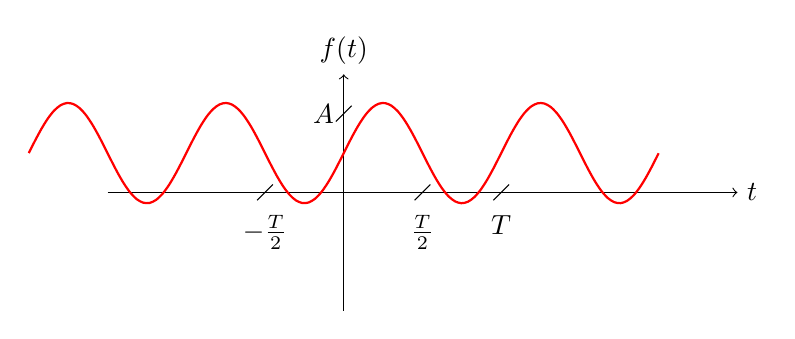
\begin{tikzpicture}
  %\draw (0,0) circle (1in);
  \draw[->] (-3.0,+0.0) -- (+5.0,+0.0) node[right] {$t$};
  \draw[->] (+0.0,-1.5) -- (+0.0,+1.5) node[above] {$f(t)$};
  %\draw[-,red, thick] (-2.5,+0.0) -- (+0.0,+0.0);
  %\draw[-] (-1.0-0.1,-0.1)--(-1.0+0.1,0.1) node[midway, below, outer sep=10pt,align=center] {$-\frac{T}{2}$};
  \draw[-] (-1.0-0.1,-0.1)--(-1.0+0.1,0.1) node[midway, below, outer sep=5pt,align=center] {$-\frac{T}{2}$};
  \draw[-] (+1.0-0.1,-0.1)--(+1.0+0.1,0.1) node[midway, below, outer sep=5pt] {$\frac{T}{2}$};
  \draw[-] (+2.0-0.1,-0.1)--(+2.0+0.1,0.1) node[midway, below, outer sep=5pt] {$T$};
  \draw[-] (-0.1,1.0-0.1)--(+0.1,1.0+0.1) node[midway, left] {$A$};
  
  \draw[scale=1.0,domain=-4:4.0,samples=100,smooth,variable=\x,red,thick] plot ({\x},{0.5+2.0/3.141592*sin(\x*180.0/3.141592*1*3.141592/1.0)});
  \end{tikzpicture}
\end{figure}

W przypadku sumowania od $k_{min}=-3$ do $k_{max}=3$ otrzymujemy 

\begin{figure}[H]
  \centering
  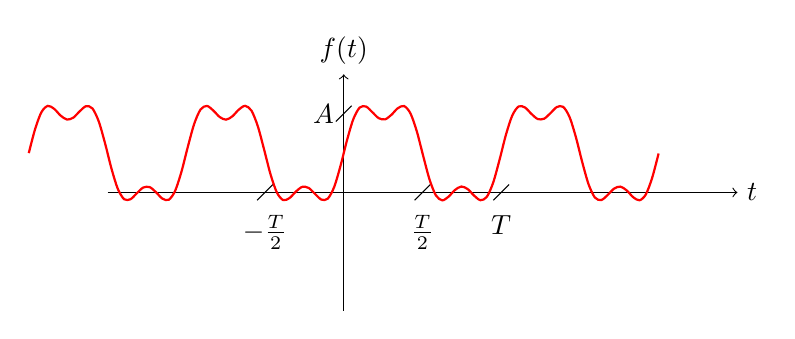
\begin{tikzpicture}
  %\draw (0,0) circle (1in);
  \draw[->] (-3.0,+0.0) -- (+5.0,+0.0) node[right] {$t$};
  \draw[->] (+0.0,-1.5) -- (+0.0,+1.5) node[above] {$f(t)$};
  %\draw[-,red, thick] (-2.5,+0.0) -- (+0.0,+0.0);
  %\draw[-] (-1.0-0.1,-0.1)--(-1.0+0.1,0.1) node[midway, below, outer sep=10pt,align=center] {$-\frac{T}{2}$};
  \draw[-] (-1.0-0.1,-0.1)--(-1.0+0.1,0.1) node[midway, below, outer sep=5pt,align=center] {$-\frac{T}{2}$};
  \draw[-] (+1.0-0.1,-0.1)--(+1.0+0.1,0.1) node[midway, below, outer sep=5pt] {$\frac{T}{2}$};
  \draw[-] (+2.0-0.1,-0.1)--(+2.0+0.1,0.1) node[midway, below, outer sep=5pt] {$T$};
  \draw[-] (-0.1,1.0-0.1)--(+0.1,1.0+0.1) node[midway, left] {$A$};
  
  \draw[scale=1.0,domain=-4:4.0,samples=100,smooth,variable=\x,red,thick] plot ({\x},{0.5+2.0/3.141592*sin(\x*180.0/3.141592*1*3.141592/1.0)+2.0/(3*3.141592)*sin(\x*180.0/3.141592*3*3.141592/1.0)});
  \end{tikzpicture}
\end{figure}

W przypadku sumowania od $k_{min}=-5$ do $k_{max}=5$ otrzymujemy 

\begin{figure}[H]
  \centering
  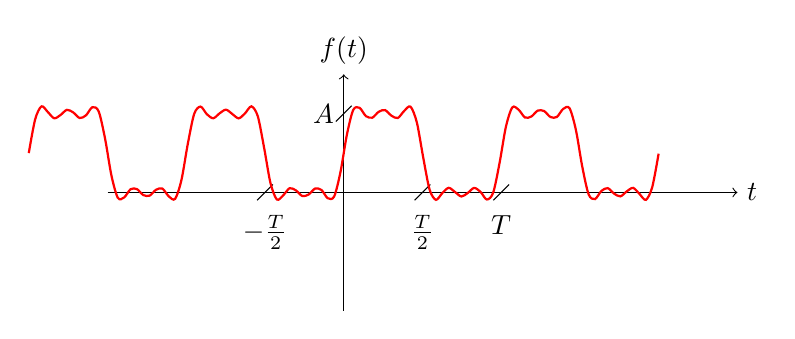
\begin{tikzpicture}
  %\draw (0,0) circle (1in);
  \draw[->] (-3.0,+0.0) -- (+5.0,+0.0) node[right] {$t$};
  \draw[->] (+0.0,-1.5) -- (+0.0,+1.5) node[above] {$f(t)$};
  %\draw[-,red, thick] (-2.5,+0.0) -- (+0.0,+0.0);
  %\draw[-] (-1.0-0.1,-0.1)--(-1.0+0.1,0.1) node[midway, below, outer sep=10pt,align=center] {$-\frac{T}{2}$};
  \draw[-] (-1.0-0.1,-0.1)--(-1.0+0.1,0.1) node[midway, below, outer sep=5pt,align=center] {$-\frac{T}{2}$};
  \draw[-] (+1.0-0.1,-0.1)--(+1.0+0.1,0.1) node[midway, below, outer sep=5pt] {$\frac{T}{2}$};
  \draw[-] (+2.0-0.1,-0.1)--(+2.0+0.1,0.1) node[midway, below, outer sep=5pt] {$T$};
  \draw[-] (-0.1,1.0-0.1)--(+0.1,1.0+0.1) node[midway, left] {$A$};
  
  \draw[scale=1.0,domain=-4:4.0,samples=100,smooth,variable=\x,red,thick] plot ({\x},{0.5+2.0/3.141592*sin(\x*180.0/3.141592*1*3.141592/1.0)+2.0/(3*3.141592)*sin(\x*180.0/3.141592*3*3.141592/1.0)+2.0/(5*3.141592)*sin(\x*180.0/3.141592*5*3.141592/1.0)});
  \end{tikzpicture}
\end{figure}

W przypadku sumowania od $k_{min}=-11$ do $k_{max}=11$ otrzymujemy 

\begin{figure}[H]
  \centering
  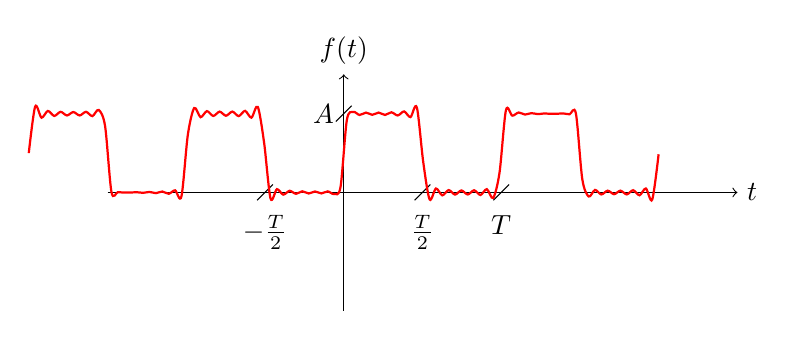
\begin{tikzpicture}
  %\draw (0,0) circle (1in);
  \draw[->] (-3.0,+0.0) -- (+5.0,+0.0) node[right] {$t$};
  \draw[->] (+0.0,-1.5) -- (+0.0,+1.5) node[above] {$f(t)$};
  %\draw[-,red, thick] (-2.5,+0.0) -- (+0.0,+0.0);
  %\draw[-] (-1.0-0.1,-0.1)--(-1.0+0.1,0.1) node[midway, below, outer sep=10pt,align=center] {$-\frac{T}{2}$};
  \draw[-] (-1.0-0.1,-0.1)--(-1.0+0.1,0.1) node[midway, below, outer sep=5pt,align=center] {$-\frac{T}{2}$};
  \draw[-] (+1.0-0.1,-0.1)--(+1.0+0.1,0.1) node[midway, below, outer sep=5pt] {$\frac{T}{2}$};
  \draw[-] (+2.0-0.1,-0.1)--(+2.0+0.1,0.1) node[midway, below, outer sep=5pt] {$T$};
  \draw[-] (-0.1,1.0-0.1)--(+0.1,1.0+0.1) node[midway, left] {$A$};
  
  \draw[scale=1.0,domain=-4:4.0,samples=100,smooth,variable=\x,red,thick] plot ({\x},{0.5+2.0/3.141592*sin(\x*180.0/3.141592*1*3.141592/1.0)+2.0/(3*3.141592)*sin(\x*180.0/3.141592*3*3.141592/1.0)+2.0/(5*3.141592)*sin(\x*180.0/3.141592*5*3.141592/1.0)+2.0/(7*3.141592)*sin(\x*180.0/3.141592*7*3.141592/1.0)+2.0/(9*3.141592)*sin(\x*180.0/3.141592*9*3.141592/1.0)+2.0/(11*3.141592)*sin(\x*180.0/3.141592*11*3.141592/1.0)});
  \end{tikzpicture}
\end{figure}

W przypadku sumowania od $k_{min}=-21$ do $k_{max}=21$ otrzymujemy 

\begin{figure}[H]
  \centering
  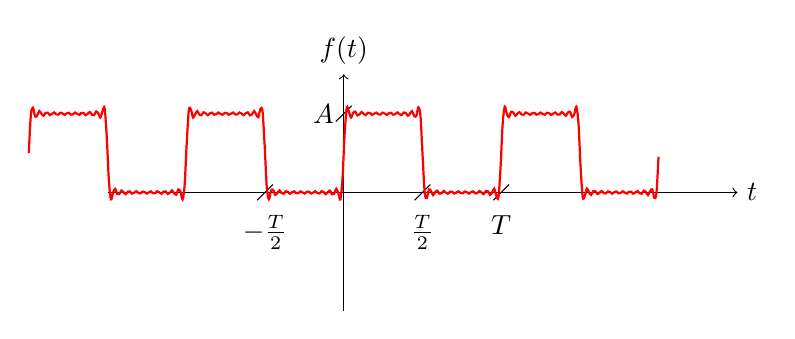
\begin{tikzpicture}
  %\draw (0,0) circle (1in);
  \draw[->] (-3.0,+0.0) -- (+5.0,+0.0) node[right] {$t$};
  \draw[->] (+0.0,-1.5) -- (+0.0,+1.5) node[above] {$f(t)$};
  %\draw[-,red, thick] (-2.5,+0.0) -- (+0.0,+0.0);
  %\draw[-] (-1.0-0.1,-0.1)--(-1.0+0.1,0.1) node[midway, below, outer sep=10pt,align=center] {$-\frac{T}{2}$};
  \draw[-] (-1.0-0.1,-0.1)--(-1.0+0.1,0.1) node[midway, below, outer sep=5pt,align=center] {$-\frac{T}{2}$};
  \draw[-] (+1.0-0.1,-0.1)--(+1.0+0.1,0.1) node[midway, below, outer sep=5pt] {$\frac{T}{2}$};
  \draw[-] (+2.0-0.1,-0.1)--(+2.0+0.1,0.1) node[midway, below, outer sep=5pt] {$T$};
  \draw[-] (-0.1,1.0-0.1)--(+0.1,1.0+0.1) node[midway, left] {$A$};
  
  \draw[scale=1.0,domain=-4:4.0,samples=300,smooth,variable=\x,red,thick] plot ({\x},{0.5+2.0/3.141592*sin(\x*180.0/3.141592*1*3.141592/1.0)+2.0/(3*3.141592)*sin(\x*180.0/3.141592*3*3.141592/1.0)+2.0/(5*3.141592)*sin(\x*180.0/3.141592*5*3.141592/1.0)+2.0/(7*3.141592)*sin(\x*180.0/3.141592*7*3.141592/1.0)+2.0/(9*3.141592)*sin(\x*180.0/3.141592*9*3.141592/1.0)+2.0/(11*3.141592)*sin(\x*180.0/3.141592*11*3.141592/1.0)+2.0/(13*3.141592)*sin(\x*180.0/3.141592*13*3.141592/1.0)+2.0/(15*3.141592)*sin(\x*180.0/3.141592*15*3.141592/1.0)+2.0/(17*3.141592)*sin(\x*180.0/3.141592*17*3.141592/1.0)+2.0/(19*3.141592)*sin(\x*180.0/3.141592*19*3.141592/1.0)+2.0/(21*3.141592)*sin(\x*180.0/3.141592*21*3.141592/1.0)});
  \end{tikzpicture}
\end{figure}

W granicy sumowania od $k_{min}=-\infty$ do $k_{max}=\infty$ otrzymujemy oryginalny sygnał.

\end{task}